\subsubsection{Energie}
\begin{itemize}
	\item Die Energie ist eine Zustandsgrösse eines Systems, die zunimmt, wenn von aussen Arbeit am System verrichtet wird, und die abnimmt, wenn das System nach aussen Arbeit verrichtet.
	\item Energieerhaltungssatz: Die Gesamtenergie $E_{tot}$ in einem abgeschlossenen System hat einen konstanten Wert, der von Vorgängern im Symsten nicht beeinfluss wird.
	\item Die Ausdehnung einer Feder ist proportional zur Kraft
	\item \textbf{Rollen auf der schiefen Ebene}: $E_{pot} = E_{kin} + E_{rot}$
\end{itemize}
\begin{tabbing}
	\begin{tabu} to \linewidth {l X l X}
		\toprule
		Energie & $E = P \cdot t$ & Rotationsenergie & $E_{rot} = \frac{J}{2} \cdot \omega^2 $\\
		Kinetische Energie & $E_{kin} = \frac{1}{2}mv^2$ &
		Potentielle Energie & $E_{pot} = F_G \cdot h =  mgh$ \\
		Federenergie & $E_f = \frac{F \cdot s}{2} = \frac{k \cdot s^2}{2}$ &
		Federkonstante & $k = \frac{F}{s}$ \\
	\end{tabu}
\end{tabbing}

\begin{tabbing}
	\begin{tabu} to \linewidth {l X l}
		Variable & Bedeutung & SI-Einheit \\
		\midrule
		$E$ & Energie & $J = Nm = Ws = \frac{kg \cdot m^2}{s^2}$ \\
		$k$ & Federkonstante & $\frac{N}{m}$  \\
		$s$ & Strecke welche die Feder ausgedehnt wird & $m$ \\
		$J$ & Trägheitsmoment & $J = kg \cdot m^2$ \\
		\bottomrule
	\end{tabu}
\end{tabbing}

\begin{minipage}[h!]{0.4\linewidth}
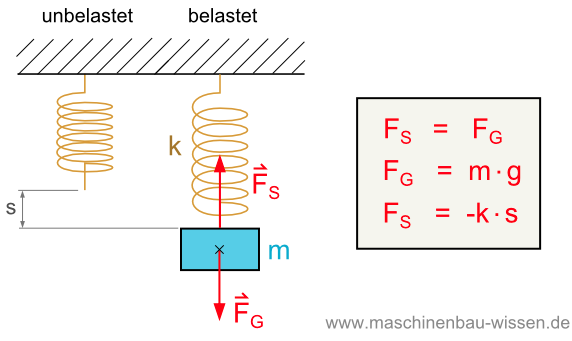
\includegraphics[width=\linewidth]{images/federenergie}
\end{minipage}
\hfill
\begin{minipage}[h!]{0.2\linewidth}
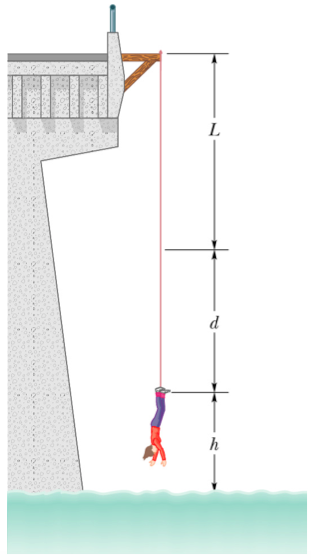
\includegraphics[width=\linewidth]{images/energie}
\end{minipage}
\hfill
\begin{minipage}[h!]{0.3\linewidth}
	\begin{align*}
	E_{pot} = E_f + E_{kin} \\
	m g (L + d) = \frac{kd^2}{2}  + \frac{m v^2}{2}  \\
	v_{Kehrpunkt} = 0 \\
	\frac{2mgL + 2mgd}{k} = d^2 \\
	d = \frac{m g}{k} \pm \frac{\sqrt{g^2 m^2 + 2 g k L m}}{k} \\
	\end{align*}
\end{minipage}
